% Copyright (c) 2016 The ALF project.
% This is a part of the ALF project documentation.
% The ALF project documentation by the ALF contributors is licensed
% under a Creative Commons Attribution-ShareAlike 4.0 International License.
% For the licensing details of the documentation see license.CCBYSA.
% !TEX root = Doc.tex
%-------------------------------------------------------------------------------------
\subsection{Performance, memory requirements and parallelization}
%-------------------------------------------------------------------------------------


As mentioned in the  introduction, the auxiliary field QMC algorithm scales linearly in inverse temperature $\beta$ and cubic in the volume $N_{\text{dim}}$. Using fast updates,  a single spin flip  requires $(N_{\text{dim}})^2$ operations to update the Green function upon acceptance.  As there are $L_{\text{Trotter}}\times N_{\text{dim}}$ spins to be visited, the total computational cost for one sweep is of the order of $\beta (N_{\text{dim}})^3$. This operation  dominates the performance, see Fig.~\ref{fig_scaling_size}. A profiling analysis of our code shows that 80-90\% of the CPU time is spend in ZGEMM calls of the BLAS library provided in the MKL package by Intel. Consequently, the single-core performance is next to optimal.

\begin{figure}[h]
	\begin{center}
		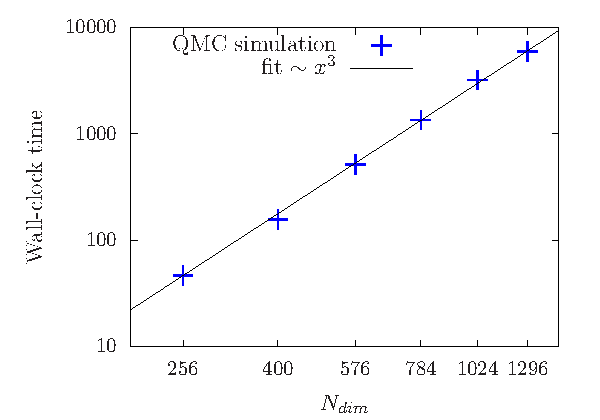
\includegraphics[scale=.8]{Figures/Size_scaling_ALF_2.pdf}
	\end{center}
	\caption{\label{fig_scaling_size}Volume scaling behavior of the auxiliary field QMC code of the ALF project on SuperMUC (phase 2/Haswell nodes) at the LRZ in Munich. The number of sites $N_{\text{dim}}$ corresponds to the system volume.
	The plot confirms that the leading scaling order is due to matrix multiplications such that the runtime is dominated by calls to ZGEMM. }
\end{figure}

For the implementation which scales linearly in $\beta$, one has to store $L_{\text{Trotter}}/\texttt{NWrap}$ intermediate propagation matrices of dimension $N\times N$. For large lattices and/or low temperatures this dominates the total memory requirements that can exceed 2~GB memory for a sequential version.

At the heart of Monte Carlo schemes lies a random walk through the given configuration space. This is easily parallalized via MPI by associating one random walker to each MPI task. For each task, we start from a random configuration and have to invest the autocorrelation time $T_\mathrm{auto}$ to produce an equilibrated configuration.
Additionally we can also profit from an OpenMP parallelized version of the BLAS/LAPACK library for an additional speedup, which also effects equilibration overhead $N_\text{MPI}\times T_\text{auto} / N_\text{OMP}$, where $N_{\text{MPI}}$ is the number of cores and $N_{\text{OMP}}$ the number of OpenMP threads.
For a given number of independent measurements  $N_\text{meas}$, we  therefore need a wall-clock time given by
\begin{equation}\label{eqn:scaling}
T  =  \frac{T_\text{auto}}{N_\text{OMP}} \left( 1   +    \frac{N_\text{meas}}{N_\text{MPI}}  \right) \,.
\end{equation}
As we typically have $ N_\text{meas}/N_\text{MPI} \gg 1 $, 
the speedup is expected to be almost perfect, in accordance with
the performance test results for the auxiliary field
QMC code  on SuperMUC (see Fig.~\ref{fig_scaling} (left)).

For many problem sizes, 2~GB memory per MPI task (random walker) suffices such that we typically start as many MPI tasks as there are physical cores per node. Due to the large amount of CPU time spent in MKL routines, we do not profit from the hyper-threading option. For large systems, the memory requirement increases and this is tackled by increasing the amount of OpenMP threads to decrease the stress on the memory system and to simultaneously reduce the equilibration overhead (see Fig.~\ref{fig_scaling} (right)). For the displayed speedup, it was crucial to pin the MPI tasks as well as the OpenMP threads in a pattern which keeps the threads as compact as possible to profit from a shared cache. This also explains the drop in efficiency from 14 to 28 threads where the OpenMP threads are spread over both sockets. 

We store the field configurations of the random walker as checkpoints, such that a long simulation can be easily split into several short simulations. This procedure allows us to take advantage of chained jobs using the dependency chains provided by the batch system.

\begin{figure}[H]
	\begin{center}
		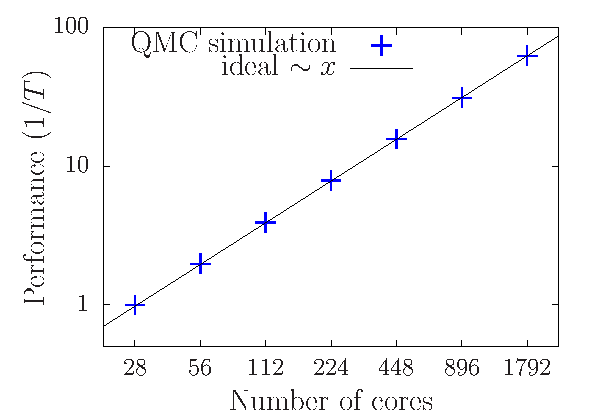
\includegraphics[scale=0.6]{Figures/MPI_scaling_ALF_2.pdf}
		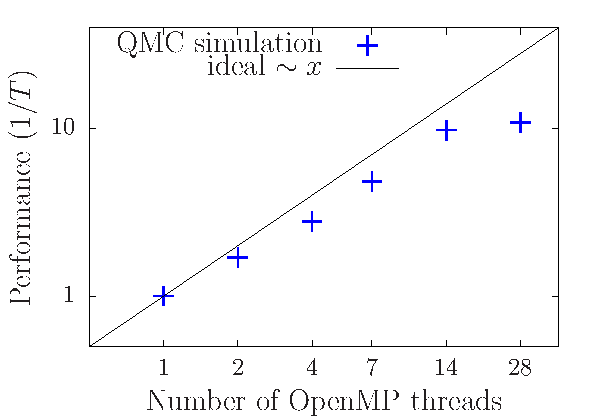
\includegraphics[scale=0.6]{Figures/OMP_scaling_ALF_2.pdf}
	\end{center}
	\caption{\label{fig_scaling} MPI (left) and OpenMP (right) scaling behavior of the auxiliary field QMC code of the ALF project on SuperMUC (phase 2/Haswell nodes) at the LRZ in Munich.
		The MPI performance data was normalized to 28 cores and was obtained using a problem size of $N_{\text{dim}}=400$. This is a medium to small system size that is the least favorable in terms of MPI synchronization effects.
		The OpenMP performance data was obtained using a problem size of $N_{\text{dim}}=1296$. Employing 2 and 4 OpenMP threads introduces some synchronization/management overhead such that the per-core performance is slightly reduced, compared to the single thread efficiency. Further increasing the amount of threads to 7 and 14 keeps the efficiency constant. The drop in performance of the 28 thread configuration is due to the architecture as the threads are now spread over both sockets of the node. To obtain the above results, it was crucial to pin the processes in a fashion that keeps the OpenMP threads as compact as possible.}
\end{figure}

%Next to the entire computational time is spent in BLAS routines such that the performance of the code will depend on the particular  implementation of this library. 
%We have found that the code performs well, and that  an efficient  OpenMP  version of the library  can be obtained merely by   loading the corresponding BLAS and LAPACK routines. 
%\mycomment{MB: Do we want to say more about OpenMP here, i.e. that it can be useful when warm-up time is a problem (and getting many CPUs is not). 
%In all other cases, the MPI parallelization is always better than the trivial OpenMP parallelization of library algos.}
